% System design document, built from design/*.md.
% Build: latexmk -pdf System_Design.tex  (then latexmk -c to remove the aux files)
\documentclass[11pt,a4paper]{report}

\usepackage[T1]{fontenc}
\usepackage[utf8]{inputenc}
\usepackage{lmodern}
\usepackage[scaled=0.88]{beramono}
\usepackage{microtype}
\usepackage[margin=2.3cm,headheight=14pt]{geometry}
\usepackage[dvipsnames,table]{xcolor}
\usepackage{array,booktabs,tabularx,xltabular}
\usepackage{enumitem}
\usepackage{listings}
\usepackage{tikz}
\usetikzlibrary{arrows.meta,positioning,shapes.geometric,calc,fit,backgrounds}
\usepackage{caption}
\usepackage{titlesec}
\usepackage{fancyhdr}
\usepackage[most]{tcolorbox}
\usepackage[hidelinks]{hyperref}

% ----- Colours -----
\definecolor{accent}{HTML}{1F4E79}
\definecolor{stable}{HTML}{D6E4F0}
\definecolor{transitional}{HTML}{FFF2CC}
\definecolor{abortc}{HTML}{F8D7DA}
\definecolor{codebg}{HTML}{F5F7FA}
\definecolor{rule}{HTML}{8EA9C1}
\definecolor{decided}{HTML}{2E7D32}
\definecolor{assumed}{HTML}{B26A00}

% ----- Layout -----
\setlength{\parindent}{0pt}
\setlength{\emergencystretch}{3em}
\setlength{\parskip}{0.55em}
\setlist{itemsep=0.15em,topsep=0.3em}
\titleformat{\chapter}[hang]{\Huge\bfseries\color{accent}}{\thechapter}{0.6em}{}
\titlespacing*{\chapter}{0pt}{-1.2em}{1.2em}
\titleformat{\section}{\Large\bfseries\color{accent}}{\thesection}{0.6em}{}
\titleformat{\subsection}{\large\bfseries}{\thesubsection}{0.6em}{}
\pagestyle{fancy}
\fancyhf{}
\fancyhead[L]{\small\color{gray}Machine Control System: Design}
\fancyhead[R]{\small\color{gray}\leftmark}
\fancyfoot[C]{\small\thepage}
\renewcommand{\headrulewidth}{0.4pt}
\fancypagestyle{plain}{\fancyhf{}\fancyfoot[C]{\small\thepage}\renewcommand{\headrulewidth}{0pt}}
\renewcommand{\arraystretch}{1.25}
\captionsetup{font=small,labelfont=bf}

% ----- Inline code and tags -----
\DeclareRobustCommand{\code}[1]{\texttt{\detokenize{#1}}}
\newcommand{\st}[1]{\textbf{#1}}                  % state name
\newcommand{\decided}{\textcolor{decided}{\textbf{Decided}}}
\newcommand{\assumed}{\textcolor{assumed}{\textbf{Assumed}}}
\newcolumntype{L}{>{\raggedright\arraybackslash}X}
\newcolumntype{P}[1]{>{\raggedright\arraybackslash}p{#1}}

% ----- Code blocks: IEC 61131-3 Structured Text -----
\lstdefinelanguage{IECST}{
  morekeywords={IF,THEN,ELSIF,ELSE,END_IF,CASE,OF,END_CASE,FOR,TO,DO,END_FOR,AND,OR,NOT,
    VAR,VAR_INPUT,VAR_OUTPUT,VAR_IN_OUT,END_VAR,TRUE,FALSE,FUNCTION_BLOCK,METHOD,INTERFACE},
  sensitive=true, morecomment=[l]{//}, morestring=[b]'}
\lstset{language=IECST, basicstyle=\ttfamily\small, keywordstyle=\color{accent}\bfseries,
  commentstyle=\color{gray}\itshape, backgroundcolor=\color{codebg}, frame=single,
  rulecolor=\color{rule}, framesep=6pt, xleftmargin=6pt, xrightmargin=6pt, columns=fullflexible,
  keepspaces=true, showstringspaces=false, breaklines=true, breakatwhitespace=true,
  postbreak=\mbox{\textcolor{gray}{$\hookrightarrow$}\space}, aboveskip=0.8em, belowskip=0.6em, upquote=true}

% ----- Callout box -----
\newtcolorbox{keypoint}[1][]{colback=stable!45,colframe=accent,boxrule=0.5pt,arc=2pt,
  left=6pt,right=6pt,top=4pt,bottom=4pt,fonttitle=\bfseries,#1}

% ----- Diagram styles -----
\tikzset{
  >={Stealth[length=2.6mm]},
  sstate/.style={draw=accent,fill=stable,rounded corners=3pt,minimum width=2.3cm,
    minimum height=0.85cm,font=\small\bfseries,align=center},
  tstate/.style={sstate,fill=transitional},
  astate/.style={sstate,fill=abortc},
  block/.style={draw=accent,fill=stable!60,rounded corners=2pt,minimum height=1cm,
    font=\small,align=center,inner xsep=6pt},
  gvl/.style={block,fill=transitional,sharp corners},
  tr/.style={->,draw=accent!80!black,thick},
  lbl/.style={font=\scriptsize,fill=white,inner sep=1.5pt,align=center},
}

\begin{document}

% =====================================================================
\begin{titlepage}
  \centering
  \vspace*{3.5cm}
  {\color{accent}\rule{\linewidth}{1.2pt}}\\[1.2em]
  {\Huge\bfseries Machine Control System\\[0.4em]}
  {\LARGE System Design\\[1.0em]}
  {\color{accent}\rule{\linewidth}{1.2pt}}\\[2em]
  {\large Central machine state management\\[0.3em]
   Servo station \quad$\cdot$\quad Drive hardware station\\[3em]}
  {\large ctrlX CORE PLC (IEC 61131-3 Structured Text)\\[0.5em]}
  \vfill
  {\large Draft for review\\[0.3em] 9 October 2026\\[0.8em]}
  {\small\color{gray}Generated from the design documents in \code{design/}. Those Markdown
   files remain the source of truth.}
\end{titlepage}

\tableofcontents

% =====================================================================
\chapter{Overview}

This document describes the control design of the machine: one central state manager that
owns the machine's operating state, and the units that follow it. The design is
\textbf{library-agnostic on purpose}. It says \emph{what} each block commands. The motion and
I/O libraries are chosen when the code is written.

\section{Documents and status}

\begin{xltabular}{\linewidth}{P{3.6cm} L P{3.6cm}}
\toprule
\textbf{Part} & \textbf{Covers} & \textbf{Status} \\
\midrule
Central state management (Ch.~\ref{ch:central}) &
\code{FB_StateManager}, the broadcast machine state, \code{I_StateClient},
\code{FB_StateClient}, \code{FB_StateRequest}, echo and done, abort jumps &
No open questions. 4 assumptions to confirm. \\
Servo station (Ch.~\ref{ch:servo}) &
\code{FB_ServoAxisMgr} (power, faults, reset, torque-free at the end of Aborting),
\code{FB_ServoMotionSeq} (position, gear-in, VM speed, hold, stop, abort) &
No open questions. 4 assumptions to confirm. \\
Drive hardware station (Ch.~\ref{ch:drive}) &
\code{FB_DriveSupplyMgr}: DC bus supply on/off from drive status bits 15/14, bit-13 fault
aborts, reset & Complete \\
\bottomrule
\end{xltabular}

\section{System structure}

\begin{figure}[h]
\centering
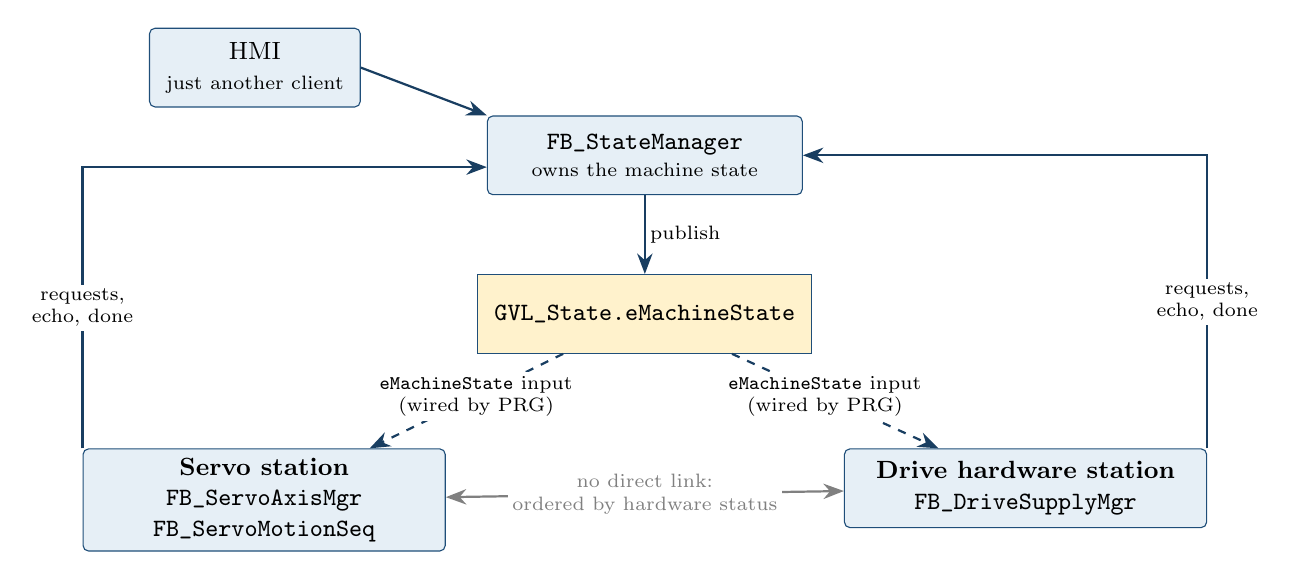
\begin{tikzpicture}[node distance=0.9cm and 1.1cm]
  \node[block,minimum width=4cm] (sm) {\code{FB_StateManager}\\[-1pt]\scriptsize owns the machine state};
  \node[gvl,below=1.0cm of sm] (gvl) {\code{GVL_State.eMachineState}};
  \node[block,below left=1.2cm and 0.4cm of gvl,minimum width=4.6cm] (servo)
     {\textbf{Servo station}\\\code{FB_ServoAxisMgr}\\\code{FB_ServoMotionSeq}};
  \node[block,below right=1.2cm and 0.4cm of gvl,minimum width=4.6cm] (drive)
     {\textbf{Drive hardware station}\\\code{FB_DriveSupplyMgr}};
  \node[block,above left=0.1cm and 1.6cm of sm,minimum width=2.4cm] (hmi) {HMI\\\scriptsize just another client};
  \draw[tr] (sm) -- node[lbl,right]{publish} (gvl);
  \draw[tr,dashed] (gvl) -- node[lbl,pos=0.45]{\code{eMachineState} input\\(wired by PRG)} (servo);
  \draw[tr,dashed] (gvl) -- node[lbl,pos=0.45]{\code{eMachineState} input\\(wired by PRG)} (drive);
  \draw[tr] (servo.north west) |- node[lbl,pos=0.25]{requests,\\echo, done} ($(sm.west)+(0,-0.15)$);
  \draw[tr] (drive.north east) |- node[lbl,pos=0.25]{requests,\\echo, done} (sm.east);
  \draw[tr] (hmi.east) -- (sm.north west);
  \draw[<->,thick,draw=gray] (servo) -- node[lbl,text=gray]{no direct link:\\ordered by hardware status} (drive);
\end{tikzpicture}
\caption{Requests go up through the clients. The state comes down through the broadcast, which
the calling program wires into each unit's \code{eMachineState} input.}
\end{figure}

\section{Implementation order}

\begin{enumerate}
  \item \textbf{Central state management:} \code{E_MachineState}, \code{I_StateClient},
        \code{FB_StateClient}, \code{FB_StateRequest}, \code{FB_StateManager} and
        \code{GVL_State}. Everything else depends on these.
  \item \textbf{Drive hardware station:} \code{FB_DriveSupplyMgr}. It has no motion and relies
        only on status words, so it's the simplest unit to bring up first.
  \item \textbf{Servo station:} \code{FB_ServoAxisMgr}, then \code{FB_ServoMotionSeq}.
  \item \textbf{Wiring:} a program that calls the manager and the units, assigns client indexes
        (\code{CLIENT_*} constants) and maps the hardware I/O (status words, supply signals,
        axis references).
\end{enumerate}

\section{Rules every implementation follows}

These come from the house style:
\begin{itemize}
  \item \textbf{Sequences use four sections:} jumps $\rightarrow$ transitions (\code{CASE},
        transitions only) $\rightarrow$ on change (\code{IF _eState <> _eLastState}: common
        actions, then entry actions) $\rightarrow$ cyclic (sub-FB calls, then all outputs last:
        command values as expressions of the state and copies of internal values).
  \item \textbf{No rising edges.} Commands are levels. A terminal state holds until its command
        is removed.
  \item \textbf{A POU never reads its own outputs.} The logic works on internal \code{_}
        variables, and the outputs are copies written at the end.
  \item \textbf{No first-scan logic.} Every state machine starts in its default (Off/Idle) state,
        which does nothing.
  \item \textbf{Enums vs constants:} an enum when the state is an output, \code{VAR CONSTANT}
        steps when it's internal. Implicit numbering, no gaps.
  \item \textbf{Any fault aborts.} Fault info is kept from the first cause and cleared on
        entering Idle.
  \item \textbf{Units never talk to each other.} They follow the broadcast state, report through
        their client, and order themselves by hardware status (e.g.\ drive status words).
  \item \textbf{No global data in an FB.} An FB never reads or writes a global variable. Global
        constants are allowed. The machine state reaches each unit through its
        \code{eMachineState} input, wired by the calling program, so another layer of state
        management can be added later without changing the units.
\end{itemize}

\section{Still to confirm}

\begin{itemize}
  \item The four assumptions of the central state management (\S\ref{sec:central-open}) and the
        four of the servo station (\S\ref{sec:servo-decisions}).
  \item The motion library has been chosen for implementation. How it provides the gear-in
        slave offset and the on-the-fly VM speed is settled in the code.
\end{itemize}

% =====================================================================
\chapter{Central Machine State Management}\label{ch:central}

\section{Purpose and scope}

One central \textbf{state manager}, \code{FB_StateManager}, owns the operating state of the
whole machine. Each unit (axis group, conveyor, heater, station, HMI\ldots) has an
\code{FB_StateClient} attached and talks to the manager only through it, using the standard
\code{FB_StateRequest} wrapper (\S\ref{sec:clients}).

\begin{keypoint}
\begin{itemize}[leftmargin=1.2em]
  \item \textbf{The state is broadcast.} The manager publishes one value,
        \code{GVL_State.eMachineState}. Each unit receives it as an \code{eMachineState}
        \textbf{input}, which the calling program wires to the broadcast. Units never read the
        GVL themselves (open question~7).
  \item \textbf{The client carries only requests upward.} The unit uses it to echo the state
        it's acting on, report done, and make requests (abort, hold, \ldots).
\end{itemize}
\end{keypoint}

The manager reads all clients each scan, decides the state and publishes it. Units never talk
to the manager or to each other directly.

\begin{minipage}[t]{0.48\linewidth}
\textbf{The state manager owns:}
\begin{itemize}
  \item the machine state and every transition between states;
  \item the rules for which requests act in which states;
  \item timeouts on the transitional states;
  \item recording the first abort cause and which client raised it.
\end{itemize}
\end{minipage}\hfill
\begin{minipage}[t]{0.48\linewidth}
\textbf{It does not own:}
\begin{itemize}
  \item \emph{how} a unit turns on, starts, stops, holds or aborts. That logic lives in the
        unit.
  \item Safety functions. E-stop, guard and STO circuits are handled by the safety system. The
        safety status reaches the manager only as an abort request, from a client owned by the
        safety-monitoring unit.
\end{itemize}
\end{minipage}

\section{States}

\begin{xltabular}{\linewidth}{P{2.2cm} P{2.1cm} L L}
\toprule
\textbf{State} & \textbf{Kind} & \textbf{Meaning} & \textbf{What the units do} \\
\midrule
\endhead
\st{Off} & Stable (default) & The machine is de-energised. This is the power-up state. & Everything is off and safe. \\
\st{TurningOn} & Transitional & The machine is bringing systems up. & Power drives, enable heaters, establish comms\ldots \\
\st{Idle} & Stable & Everything is on and ready, but no production. There's no fault in Idle. & Hold ready. No motion. \\
\st{Starting} & Transitional & Preparing for production. & Home or move to start positions, ramp up, prime\ldots \\
\st{Running} & Stable & Producing. & Normal cyclic operation. \\
\st{Stopping} & Transitional & Controlled stop at the end of a cycle. & Finish the current cycle and bring to rest. \\
\st{Holding} & Transitional & Pausing production in a resumable way. & Pause at a safe point and keep position and context. \\
\st{Hold} & Stable & Paused, and production can resume. & Stay paused. \\
\st{UnHolding} & Transitional & Resuming from Hold. & Restore motion and context. \\
\st{Aborting} & Transitional & Fast stop because something is wrong. & Stop as quickly as is safe, in the shortest way. \\
\st{Aborted} & Stable & Stopped after an abort and waiting for reset. & Stay stopped and safe. \\
\st{Resetting} & Transitional & Recovering from an abort. & Clear faults, re-enable, return to a known condition. \\
\bottomrule
\end{xltabular}

Every \textbf{transitional} state has a timeout (\S\ref{sec:jumps}) and leaves when
\textbf{all clients are done} with it. \textbf{Stable} states have no timeout, and they leave
on requests.

\section{Transitions}

\code{AllDone} means every active client reports that it has finished the current state
(\S\ref{sec:manager}).

\begin{figure}[h]
\centering
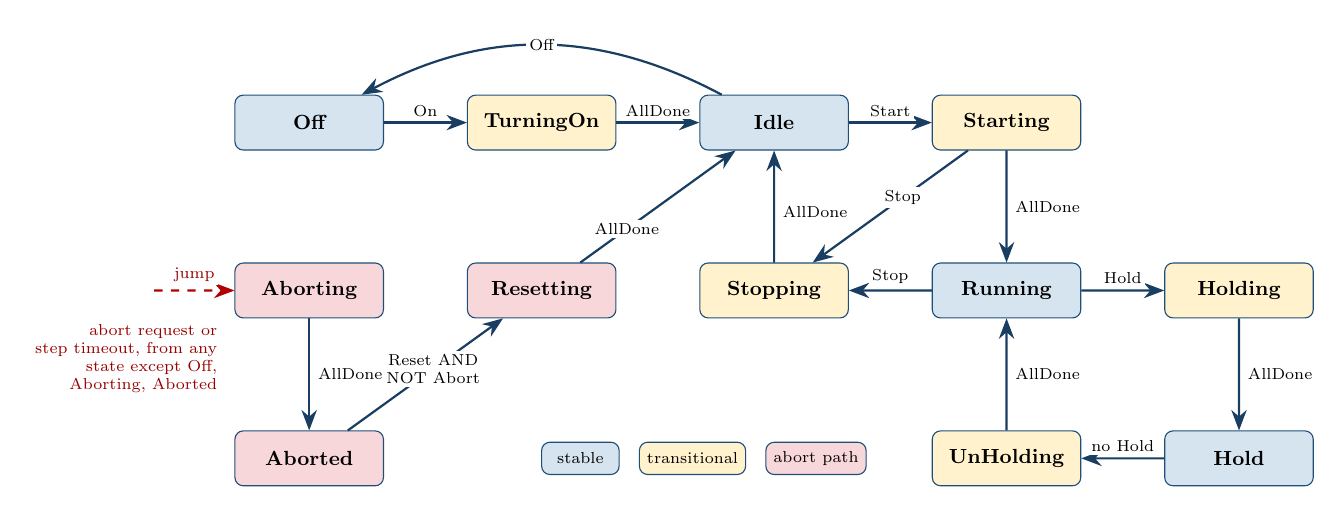
\begin{tikzpicture}[x=1cm,y=1cm,scale=0.82,transform shape]
  % stable: blue, transitional: yellow, abort path: red
  \node[sstate] (off)   at (0,0)      {Off};
  \node[tstate] (ton)   at (3.6,0)    {TurningOn};
  \node[sstate] (idle)  at (7.2,0)    {Idle};
  \node[tstate] (start) at (10.8,0)   {Starting};
  \node[tstate] (stop)  at (7.2,-2.6) {Stopping};
  \node[sstate] (run)   at (10.8,-2.6){Running};
  \node[tstate] (hing)  at (14.4,-2.6){Holding};
  \node[sstate] (hold)  at (14.4,-5.2){Hold};
  \node[tstate] (unh)   at (10.8,-5.2){UnHolding};
  \node[astate] (abing) at (0,-2.6)   {Aborting};
  \node[astate] (abed)  at (0,-5.2)   {Aborted};
  \node[astate] (reset) at (3.6,-2.6) {Resetting};

  \draw[tr] (off) -- node[lbl,above=1pt]{On} (ton);
  \draw[tr] (ton) -- node[lbl,above=1pt]{AllDone} (idle);
  \draw[tr] (idle) to[bend right=28] node[lbl]{Off} (off);
  \draw[tr] (idle) -- node[lbl,above=1pt]{Start} (start);
  \draw[tr] (start) -- node[lbl,right=2pt,pos=0.5]{AllDone} (run);
  \draw[tr] (start) -- node[lbl,pos=0.42]{Stop} (stop);
  \draw[tr] (run) -- node[lbl,above=1pt]{Stop} (stop);
  \draw[tr] (stop) -- node[lbl,right=2pt,pos=0.45]{AllDone} (idle);
  \draw[tr] (run) -- node[lbl,above=1pt]{Hold} (hing);
  \draw[tr] (hing) -- node[lbl,right=2pt]{AllDone} (hold);
  \draw[tr] (hold) -- node[lbl,above=1pt]{no Hold} (unh);
  \draw[tr] (unh) -- node[lbl,right=2pt]{AllDone} (run);
  \draw[tr] (abing) -- node[lbl,right=2pt]{AllDone} (abed);
  \draw[tr] (abed) -- node[lbl,pos=0.55]{Reset AND\\NOT Abort} (reset);
  \draw[tr] (reset) -- node[lbl,pos=0.3]{AllDone} (idle);
  \draw[tr,dashed,draw=red!70!black] (-2.4,-2.6) -- node[lbl,above=2pt,text=red!60!black]{jump} (abing);
  \node[font=\scriptsize,text=red!60!black,align=right,anchor=north east] at (-1.3,-3.0)
    {abort request or\\step timeout, from any\\state except Off,\\Aborting, Aborted};

  % legend
  \node[sstate,minimum width=1.2cm,minimum height=0.5cm,font=\scriptsize] (l1) at (4.2,-5.2) {stable};
  \node[tstate,minimum width=1.2cm,minimum height=0.5cm,font=\scriptsize,right=0.3cm of l1] (l2) {transitional};
  \node[astate,minimum width=1.2cm,minimum height=0.5cm,font=\scriptsize,right=0.3cm of l2] {abort path};
\end{tikzpicture}
\caption{Machine states. Requests are the combined (OR) requests of all clients, as levels.}
\label{fig:states}
\end{figure}

\subsection*{Transition table (normal transitions)}

\begin{center}
\begin{tabular}{l l l}
\toprule
\textbf{From} & \textbf{Condition} & \textbf{To} \\
\midrule
Off & \code{On AND NOT Off} & TurningOn \\
TurningOn & \code{AllDone} & Idle \\
Idle & \code{Off} & Off \\
Idle & \code{Start AND NOT Stop AND NOT Off} & Starting \\
Starting & \code{Stop} & Stopping \\
Starting & \code{AllDone} & Running \\
Running & \code{Stop} & Stopping \\
Running & \code{Hold} & Holding \\
Stopping & \code{AllDone} & Idle \\
Holding & \code{AllDone} & Hold \\
Hold & \code{NOT Hold} & UnHolding \\
UnHolding & \code{AllDone} & Running \\
Aborting & \code{AllDone} & Aborted \\
Aborted & \code{Reset AND NOT Abort} & Resetting \\
Resetting & \code{AllDone} & Idle \\
\bottomrule
\end{tabular}
\end{center}

\begin{itemize}
  \item \textbf{Priorities inside Running:} stop is checked before hold, so if both are
        requested the machine stops.
  \item \textbf{Stop during Starting} always goes to Stopping, whether or not starting has
        completed. Stop is checked before \code{AllDone}.
  \item \textbf{Hold lasts while any client requests it.} The machine resumes only when
        \textbf{no} client requests hold any more, so a starved infeed and an operator pause can
        overlap safely.
  \item \textbf{Off is reached only from Idle.} Going from Running to Off therefore passes
        through Stopping first.
  \item \textbf{Aborted $\rightarrow$ Resetting requires that no client still requests an abort.}
        A held abort can't be reset away.
\end{itemize}

\section{Jumps: abort and timeouts}\label{sec:jumps}

The jumps are evaluated \textbf{before} the transitions, in priority order, from every state
except Off, Aborting and Aborted:

\begin{xltabular}{\linewidth}{c P{4.6cm} c L}
\toprule
\textbf{Prio.} & \textbf{Condition} & \textbf{To} & \textbf{Recorded} \\
\midrule
1 & Any client requests an abort & Aborting & That client's abort code, the client's index, and the state it came from \\
2 & Step timer of the current transitional state has expired & Aborting & ``Timeout'', the state, the first client that wasn't done, and whether it never acknowledged or never finished (\S\ref{sec:manager}) \\
\bottomrule
\end{xltabular}

The transition \code{CASE} then runs as normal on the state the jump set. Exits from Aborting
are themselves conditions (\code{AllDone}), so a transition that fires in the same scan is a
correct one.

\textbf{Fault information:}
\begin{itemize}
  \item Only the \textbf{first} cause is recorded. The jumps aren't evaluated in Aborting or
        Aborted, so later faults can't overwrite it.
  \item \textbf{Units don't raise fault-based abort requests in Aborting, Aborted or Resetting.}
        A fault is reset \emph{in} Resetting, but Aborted $\rightarrow$ Resetting requires that no
        client requests an abort, so a fault that's still present would block its own reset. A
        fault that survives the reset leaves the unit not done, and the Resetting timeout aborts
        again. Deliberate aborts (operator, safety) keep requesting, so they still block the
        reset.
  \item The cause is \textbf{cleared on entry to Idle}. Idle means nothing is wrong, so there's
        no fault to show. The cause stays visible for the whole Aborting $\rightarrow$ Aborted
        $\rightarrow$ Resetting path.
\end{itemize}

\textbf{Timeout in Aborting.} If clients don't confirm Aborting within the abort timeout, the
machine still goes to Aborted. The client that didn't confirm is recorded as a second
diagnostic. Reaching a resettable state matters more than waiting forever.

\section{Clients: interface, client FB and wrapper}\label{sec:clients}

A client has three standard layers. They're the same for every unit.

\begin{figure}[h]
\centering
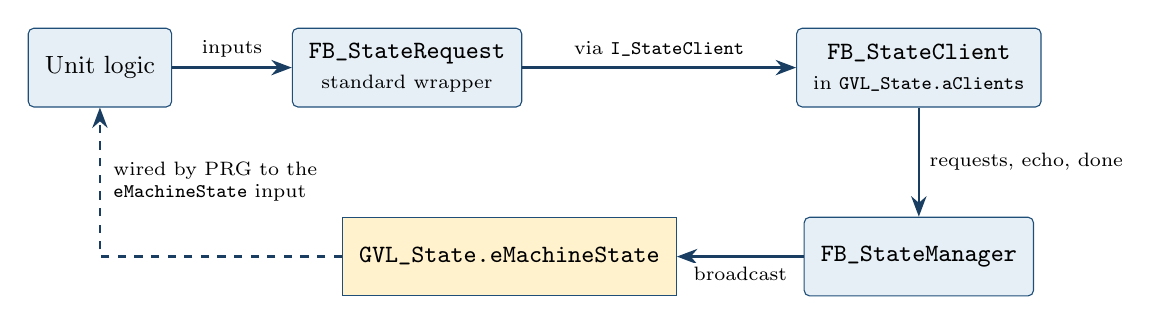
\begin{tikzpicture}[x=1cm,y=1cm]
  \node[block] (u) at (0,0)     {Unit logic};
  \node[block] (w) at (3.9,0)   {\code{FB_StateRequest}\\\scriptsize standard wrapper};
  \node[block] (c) at (10.4,0)  {\code{FB_StateClient}\\\scriptsize in \code{GVL_State.aClients}};
  \node[block] (m) at (10.4,-2.4){\code{FB_StateManager}};
  \node[gvl]   (g) at (5.2,-2.4){\code{GVL_State.eMachineState}};
  \draw[tr] (u) -- node[lbl,above=2pt]{inputs} (w);
  \draw[tr] (w) -- node[lbl,above=2pt]{via \code{I_StateClient}} (c);
  \draw[tr] (c) -- node[lbl,right=2pt]{requests, echo, done} (m);
  \draw[tr] (m) -- node[lbl,below=2pt]{broadcast} (g);
  \draw[tr,dashed] (g) -| node[lbl,pos=0.75,right=3pt,align=left]{wired by PRG to the\\\code{eMachineState} input} (u);
\end{tikzpicture}
\caption{The three client layers, and the state coming back down.}
\end{figure}

\begin{enumerate}
  \item \textbf{\code{I_StateClient} (interface).} The standard way to talk to a client: request
        levels, state echo and done, all going up to the manager.
  \item \textbf{\code{FB_StateClient IMPLEMENTS I_StateClient}.} The actual client. It stores the
        request levels, echo and done. The manager reads these instances
        (\S\ref{sec:manager}). The client doesn't carry the state; that's the broadcast.
  \item \textbf{\code{FB_StateRequest} (wrapper).} The one block a unit uses. It holds the
        attached \code{I_StateClient}, checks it isn't null, and forwards the unit's inputs
        through the interface every call. Units never touch the interface or the client
        directly, so using a client takes a single FB call.
\end{enumerate}

\subsection{\texorpdfstring{\code{I_StateClient}}{I_StateClient}}

\begin{xltabular}{\linewidth}{P{6.4cm} c L}
\toprule
\textbf{Member} & \textbf{Kind} & \textbf{Meaning} \\
\midrule
\code{Request(bOn, bOff, bStart, bStop, bHold, bAbort, uiAbortCode, bReset)} & Method & Sets this client's request levels. Every call overwrites all of them. \\
\code{Report(eStateEcho, bDone, bEnable)} & Method & The state the unit is acting on, whether it's finished, and whether the client takes part at all. \\
\bottomrule
\end{xltabular}

\subsection{\texorpdfstring{\code{FB_StateRequest}}{FB_StateRequest} (wrapper)}

\begin{xltabular}{\linewidth}{L P{4.2cm}}
\toprule
\textbf{Inputs} & \textbf{Outputs} \\
\midrule
\code{itfClient : I_StateClient}: the attached client & \code{bAttached}: \code{itfClient <> 0} \\
\code{bOn}, \code{bOff}, \code{bStart}, \code{bStop}, \code{bHold}, \code{bReset}: requests (levels, default FALSE) & \\
\code{bAbort}, \code{uiAbortCode}: abort request and its reason & \\
\code{eStateEcho}, \code{bDone}: progress on the current state & \\
\code{bEnable} (default TRUE): FALSE switches the unit out of the machine state & \\
\bottomrule
\end{xltabular}

A unit connects only the inputs it uses, and the rest stay FALSE. It's called with the unit's
other sub-FBs at the end, before the unit's outputs:

\begin{lstlisting}
_fbStateReq(
    itfClient   := itfClient,                  // wired by the caller to aClients[CLIENT_INFEED]
    bAbort      := _eState = E_InfeedState.Faulted,
    uiAbortCode := _uiFaultCode,
    bHold       := _eState = E_InfeedState.Starved,
    eStateEcho  := _eMachineStateSeen,         // machine state this unit has taken over
    bDone       := _bStepDone);
\end{lstlisting}

Inside, the wrapper does:
\begin{lstlisting}
IF itfClient <> 0 THEN itfClient.Request(...); itfClient.Report(...); END_IF
\end{lstlisting}
All requests are written every call, so releasing an input releases the request.

The unit's own state machine follows the machine state it's given: its transitions read its
\code{eMachineState} input (latched once per scan into an internal variable), and when it has
taken a machine state over it echoes that state back through the wrapper. The calling program
wires the input, normally \code{eMachineState := GVL_State.eMachineState}.

\begin{keypoint}[title={Done is the echoed state plus a done bit}]
The manager counts a client as done only when \code{eStateEcho = current state AND bDone}.
\begin{itemize}[leftmargin=1.2em]
  \item \textbf{Echo without done:} the unit has picked up the new state and is working on it.
        The manager can show which units are still busy, and a timeout can name the one that
        never acknowledged.
  \item \textbf{Echo of an old state:} the unit hasn't taken the new state over yet. Its
        \code{bDone} refers to the old state and is ignored. A stale done from Holding can never
        satisfy UnHolding.
  \item The unit sets both from its own state machine: \code{eStateEcho} follows the state it's
        actually in, and \code{bDone} comes from its own logic. Both are levels, and there's
        nothing to clear.
\end{itemize}
\end{keypoint}

\textbf{Units with nothing to do} in a state echo it and set \code{bDone} straight away. For
example, a heater has nothing to hold, so in Holding it reports done immediately.

\textbf{Commands are levels.} The HMI is just another client, so operator buttons are held
requests too. There are no rising edges anywhere: stable states wait for a request to change,
so a held request can't re-trigger anything. That works the same way as \code{Done}, which
waits for \code{Execute} to drop.

\section{The manager: how clients are combined}\label{sec:manager}

\begin{figure}[h]
\centering
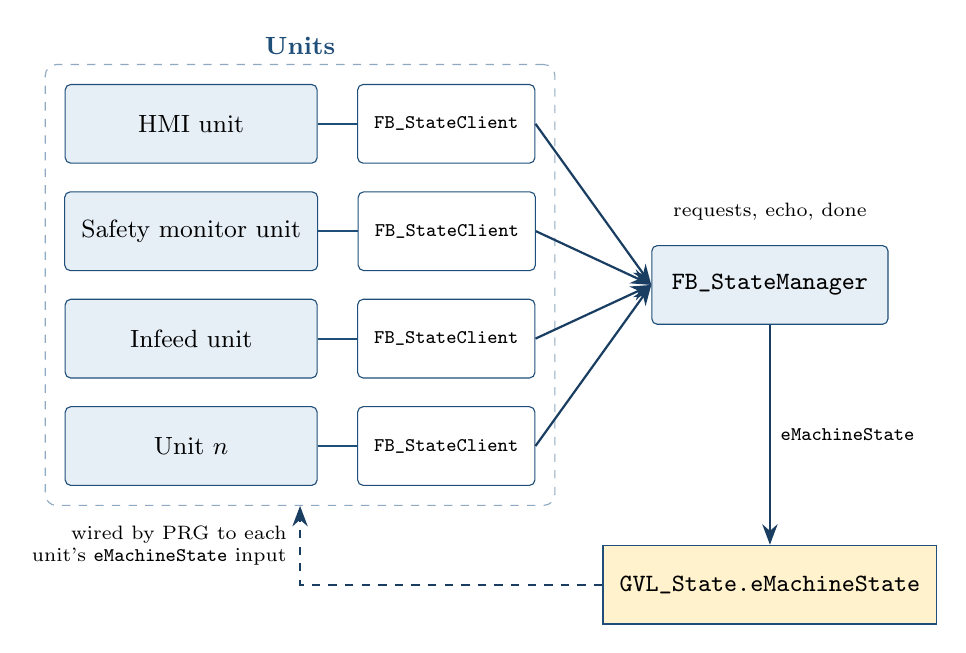
\begin{tikzpicture}[node distance=0.35cm and 0.5cm]
  \node[block,minimum width=3.2cm] (hmi) {HMI unit};
  \node[block,minimum width=3.2cm,below=of hmi] (saf) {Safety monitor unit};
  \node[block,minimum width=3.2cm,below=of saf] (inf) {Infeed unit};
  \node[block,minimum width=3.2cm,below=of inf] (un) {Unit $n$};
  \foreach \u/\i in {hmi/0,saf/1,inf/2,un/n} {
    \node[block,fill=white,right=0.5cm of \u,font=\scriptsize] (c\i) {\code{FB_StateClient}};
    \draw[thick,draw=accent] (\u) -- (c\i);
  }
  \begin{scope}[on background layer]
    \node[draw=rule,dashed,rounded corners,fit=(hmi)(cn),inner sep=7pt,
          label={[font=\small\bfseries,text=accent]above:Units}] (units) {};
  \end{scope}
  \node[block,right=2.6cm of $(c1)!0.5!(c2)$,minimum width=3cm] (sm) {\code{FB_StateManager}};
  \foreach \i in {0,1,2,n} { \draw[tr] (c\i.east) -- (sm.west); }
  \node[lbl,anchor=south] at ($(sm.north)+(0,0.25)$) {requests, echo, done};
  \node[gvl] (b) at ($(sm |- units.south)+(0,-1.0)$) {\code{GVL_State.eMachineState}};
  \draw[tr] (sm) -- node[lbl,right=2pt]{\code{eMachineState}} (b);
  \draw[tr,dashed] (b.west) -| node[lbl,pos=0.75,left=3pt,align=right]{wired by PRG to each\\unit's \code{eMachineState} input}
     (units.south);
\end{tikzpicture}
\caption{The manager combines every client, then publishes one state.}
\end{figure}

Each scan, \code{FB_StateManager} runs the house sequence structure, with one extra section in
front:

\begin{enumerate}[start=0]
  \item \textbf{Read clients.} A \code{FOR} loop over the client array builds the combined
        requests and \code{AllDone}:
  \begin{itemize}
    \item each request (\code{Abort}, \code{Hold}, \code{Stop}, \code{Start}, \code{On},
          \code{Off}, \code{Reset}) is the OR across all active clients;
    \item \code{AllDone} is the AND of \code{client.eStateEcho = _eState AND client.bDone}
          across all active clients;
    \item the loop records the \textbf{first} client requesting an abort (index and code), and
          the \textbf{first} client that isn't done. It also notes whether that client hasn't
          acknowledged (echo $\neq$ state) or is still working (echo $=$ state, not done), for
          timeout diagnostics.
  \end{itemize}
  \item \textbf{Jumps:} abort, then timeout (\S\ref{sec:jumps}).
  \item \textbf{Transitions:} a \code{CASE} with only the state changes in
        Figure~\ref{fig:states}, plus \code{ELSE} $\rightarrow$ Aborting.
  \item \textbf{On change:} \code{IF _eState <> _eLastState}. First the common actions: restart
        the step timer and clear the timeout. Then the per-state entry actions: set the timeout
        for each transitional state, and clear the abort info on entering Idle.
  \item \textbf{Cyclic:} the manager's outputs, including the broadcast \code{eMachineState},
        are copied from internal variables, and the step timer is called last.
\end{enumerate}

The clients are read at the start and the state is published at the end, so units always see
the state the manager settled on in this scan. A unit that reports done is picked up in the
manager's next scan. Data flows one way through each path: requests go up through the clients,
and the state comes down through the broadcast.

\section{Implementation notes}

\textbf{Registering clients.} There were two options (open question~1):
\begin{itemize}
  \item \textbf{A. Array passed in:} \code{VAR_IN_OUT aClients : ARRAY[*] OF FB_StateClient},
        with the array declared in a GVL (\code{GVL_State.aClients[1..MAX_CLIENTS]}). Each unit
        is given a fixed index (constant), e.g.\ \code{GVL_State.aClients[CLIENT_INFEED]}. Bounds
        come from \code{LOWER_BOUND}/\code{UPPER_BOUND}. This is simple and visible online, and
        adding a unit means adding one constant. \decided.
  \item \textbf{B. Registration by reference:} each unit's client calls
        \code{fbManager.Register(THIS^)} once, and the manager stores
        \code{REFERENCE TO FB_StateClient} in a fixed-size table. Clients live inside their
        units, but it adds init-order and online-change concerns.
\end{itemize}

\textbf{Active clients.} A client counts toward \code{AllDone} and the request ORs only while
it's enabled. \textbf{A client starts disabled}, and it becomes enabled when a unit's
\code{FB_StateRequest} reports \code{bEnable} (default TRUE). Unused slots in \code{aClients}
are therefore ignored, so they can't block \code{AllDone}. A unit that's switched out (e.g.\ an
optional station) passes \code{bEnable := FALSE} instead of reporting done everywhere.

\textbf{Types and conventions:}
\begin{itemize}
  \item \code{E_MachineState} is an enum with \code{{attribute 'qualified_only'}} and
        \code{{attribute 'strict'}}, numbered implicitly from \code{Off := 0}. It's an enum
        because the state is exposed.
  \item \textbf{Internal state:} \code{_eState}, \code{_eLastState}, \code{_uiAbortCode},
        \code{_iAbortClient} and \code{_eAbortFrom} are the manager's internal variables. The
        outputs are copies.
  \item \textbf{Timeouts and client indexes} are \code{VAR CONSTANT}s.
  \item \textbf{No first-scan logic.} The machine starts in Off, which does nothing, and every
        client's defaults (\code{eStateEcho} = Off, \code{bDone} = FALSE) are consistent with
        that.
\end{itemize}

\textbf{Manager outputs}, published to \code{GVL_State}: \code{eMachineState} (the broadcast),
plus \code{uiAbortCode}, \code{iAbortClient}, \code{eAbortFrom} and \code{iNotDoneClient} for
the HMI and diagnostics. A unit that wants to know whether it caused the abort compares
\code{iAbortClient} with its own client index.

\section{Assumptions and decisions}\label{sec:central-open}

\textbf{\assumed\ (please confirm):}
\begin{enumerate}
  \item ``someStartCmd $\rightarrow$ Start $\rightarrow$ Starting'' has been read as a single
        \st{Starting} state. There's no separate \st{Start} state.
  \item Reset leads to \textbf{Idle}: Aborted $\rightarrow$ Resetting $\rightarrow$ Idle.
  \item Abort applies from every state except Off, Aborting and Aborted.
  \item A transitional-state timeout counts as an abort, not as a separate Faulted state.
\end{enumerate}

\textbf{Open questions, all \decided:}
\begin{enumerate}
  \item \textbf{Client registration:} option A. \code{GVL_State.aClients[1..MAX_CLIENTS]}, an array of \code{FB_StateClient},
        is passed to the manager as \code{VAR_IN_OUT ARRAY[*]}, and each unit uses a
        \code{CLIENT_*} index constant.
  \item \textbf{Request policy:} all requests are equal. Every enabled client's requests are
        combined (OR) the same way, whichever client they come from.
  \item \textbf{Stop while in Hold or Holding:} not needed. Stop acts from Running only, so a held
        machine resumes first. (The servo sequence would handle a stop from any step anyway.)
  \item \textbf{Stop while Starting:} a stop request in Starting always goes to Stopping,
        whether or not starting has completed. Units must handle a stop from mid-start; the
        servo sequence does this with its stop jump.
  \item \textbf{A TurningOff state:} no. Going to Off just powers the axes down. The drive supply
        already waits until no axis is under torque before it switches off, so the order is
        right without an extra state.
  \item \textbf{Start held through a stop:} the machine just starts again. A start request still
        held when Stopping returns to Idle restarts it, as written.
  \item \textbf{How units get the broadcast state:} as an input. No FB reads or writes a global
        variable (global constants are fine). Every unit has an
        \code{eMachineState : E_MachineState} input, and only the calling program wires it to
        \code{GVL_State.eMachineState}. If the machine grows and needs another layer of state
        management (e.g.\ a sub-manager per section of the line), a unit can be given that
        sub-manager's state instead of the machine state, without any change inside the unit.
        It also makes every unit's dependencies visible at its call site.
\end{enumerate}

% =====================================================================
\chapter{Unit: Servo Station}\label{ch:servo}

\section{Purpose and scope}

The servo station has \textbf{two real servo axes} and \textbf{one virtual master (VM)}. In
production, both real axes are geared 1:1 to the VM at caller-supplied phase offsets, and the
line speed is the VM's velocity.

The unit follows the machine state it's given as its \code{eMachineState} input (wired by the
calling program to the broadcast \code{GVL_State.eMachineState}) and is split into two blocks.
Each block has its own state client (\code{FB_StateRequest}):

\begin{center}
\begin{tabularx}{\linewidth}{P{4cm} L}
\toprule
\textbf{Block} & \textbf{Job} \\
\midrule
\code{FB_ServoAxisMgr} & Axis power on/off, fault detection with abort requests, and axis fault reset. \\
\code{FB_ServoMotionSeq} & All motion: positioning, gear-in, VM speed, hold/unhold, stop and abort sequences. \\
\bottomrule
\end{tabularx}
\end{center}

The manager waits for \textbf{both} clients before it leaves a transitional state. Power and
motion therefore stay independent, and neither block needs to know the other's internals.

This chapter says \emph{what} each block commands. It doesn't commit to a motion library.
Commands are named by function (power, reset, absolute move, gear-in, velocity move, halt,
stop), and the implementation picks the library that provides them.

\section{Axes}

\begin{center}
\begin{tabularx}{\linewidth}{l P{5cm} L}
\toprule
\textbf{Name} & \textbf{Type} & \textbf{Role} \\
\midrule
\code{Ax1} & Real servo, rotary modulo 360\textdegree & Slave 1, geared 1:1 to the VM at \code{lrAx1Offset} \\
\code{Ax2} & Real servo, rotary modulo 360\textdegree & Slave 2, geared 1:1 to the VM at \code{lrAx2Offset} \\
\code{VM} & Virtual axis, rotary modulo 360\textdegree & Master. Its velocity is the line speed. \\
\bottomrule
\end{tabularx}
\end{center}

The offsets are \textbf{inputs from the caller} (\S\ref{sec:servo-if}). For the current machine
the caller passes \code{OFFSET} for Ax1 and \code{360 - OFFSET} for Ax2. The blocks don't know
or assume that relationship.

\section{\texorpdfstring{\code{FB_ServoAxisMgr}}{FB_ServoAxisMgr}: power, faults, reset}

\subsection{Behaviour per machine state}

\begin{xltabular}{\linewidth}{P{3.6cm} L P{3.6cm}}
\toprule
\textbf{Machine state} & \textbf{Axis power} & \textbf{Done when} \\
\midrule
\st{Off} & Off & All 3 axes report disabled \\
\st{TurningOn} & On, once the axis reports ready for power (see below) & All 3 powered, no axis error \\
Idle, Starting, Running, Stopping, Holding, Hold, UnHolding & On & Immediately: nothing to do beyond staying powered \\
\st{Aborting} & On while the motion block stops the axes. Once \textbf{all axes are at rest} (standstill, stopped, error-stop or disabled), they're commanded \textbf{torque-free} while the machine is still in Aborting. & All 3 report disabled (torque-free) \\
\st{Aborted} & Off & All 3 report disabled \\
\st{Resetting} & Reset both axes on entry, then on once the axes report ready for power & All 3 powered, no axis error \\
\bottomrule
\end{xltabular}

Power is a level derived from the machine state and the axis states:

\begin{lstlisting}
bWantPower   := eMachineState <> Off AND eMachineState <> Aborted
                AND NOT (eMachineState = Aborting AND bAllAxesAtRest);
bPowerEnable := bWantPower AND bPowerReady;
\end{lstlisting}

\begin{itemize}
  \item \code{bAllAxesAtRest}: every axis is in standstill, stopped, error-stop or disabled.
        ``Disabled'' is included, so once the axes are torque-free they stay torque-free for the
        rest of Aborting, with no latch needed.
  \item \code{bPowerReady}, per axis: the axis's own \textbf{ready-for-power feedback} from the
        motion system (``the drive is ready for power up''). For a real axis it only comes once
        the drive hardware station has the DC bus up, so the ordering still comes from the
        hardware status, with no unit-to-unit link. The servo station deliberately
        \textbf{doesn't read the drive status word}; the drive hardware station owns it. Because
        of that, any axis can be switched to a virtual axis for testing without changing this
        unit. \decided\ (it replaces the earlier ``drive status word bit 15'' condition).
  \item \textbf{Torque-free at the end of Aborting} is what lets the drive hardware station
        confirm that no axis is under torque and shut the supply down within Aborting
        (Chapter~\ref{ch:drive}).
  \item If the motion block's stop commands report errors because power was removed, those are
        ignored: the machine is already in Aborting, and the first abort cause has been recorded.
\end{itemize}

\subsection{Fault detection: abort requests}

\textbf{Any fault aborts.} Outside Aborting, Aborted and Resetting (\S\ref{sec:jumps}), the
block requests an abort (through its client) while any of these is TRUE:

\begin{center}
\begin{tabularx}{\linewidth}{P{4.4cm} L}
\toprule
\textbf{Abort code} & \textbf{Condition} \\
\midrule
\code{ABORT_AXIS_ERROR + i} & Axis $i$ is in its error-stop state or has a drive error \\
\code{ABORT_POWER_LOST + i} & Axis $i$ should be powered (\code{bPowerEnable} has been TRUE, outside TurningOn and Resetting) but isn't \\
\bottomrule
\end{tabularx}
\end{center}

The first matching code is reported. The central manager keeps only the first abort
machine-wide.

\subsection{Reset}

On \textbf{entry to Resetting}, a reset is issued to \textbf{both real axes}, whatever caused
the abort. Any fault aborts, so Resetting always follows a fault, and the reset doesn't need to
know which one. The axes are torque-free (disabled) at that point, which is one of the states
where the reset is allowed.
\begin{itemize}
  \item The reset of Ax1 (drive 0) also clears the drive supply, which is built into drive 0.
  \item After the reset, power comes back on as soon as the axes report ready for power.
  \item The block reports done once no axis has an error and all are powered.
  \item If an axis won't reset, the manager's Resetting timeout aborts again, with this client
        recorded as the one not done.
\end{itemize}

\subsection{Internal structure}

This block has no sequence of its own. Everything is a level function of the machine state and
the axis status, so there's no internal state machine. It's written as:
\begin{enumerate}
  \item read the axis status (results from the previous scan);
  \item fault conditions $\rightarrow$ abort request and code;
  \item echo and done from the machine state;
  \item command levels (power enable), and the reset of both axes on entry to Resetting;
  \item call the sub-FBs (power, reset and status for each axis), then copy the outputs last.
\end{enumerate}

\section{\texorpdfstring{\code{FB_ServoMotionSeq}}{FB_ServoMotionSeq}: motion sequence}

\subsection{Internal states (\texorpdfstring{\code{E_ServoSeqState}}{E_ServoSeqState})}

\begin{xltabular}{\linewidth}{P{3.1cm} L P{4.0cm}}
\toprule
\textbf{State} & \textbf{Commands (levels from this state)} & \textbf{Leaves when} \\
\midrule
\endhead
\st{Idle} & None. All axes are at standstill and ungeared. & The machine is Starting \\
\st{Positioning} & Absolute moves, all in parallel and by the shortest way: Ax1 $\rightarrow$ \code{lrAx1Offset}, Ax2 $\rightarrow$ \code{lrAx2Offset}, VM $\rightarrow$ 0 & All three done $\rightarrow$ GearingIn \\
\st{GearingIn} & Gear Ax1 and Ax2 to the VM in \textbf{absolute position mode} against the VM's \textbf{set point}, ratio 1:1, with slave offsets \code{lrAx1Offset} / \code{lrAx2Offset}, synchronising by the shortest way & Both in sync $\rightarrow$ Synced \\
\st{Synced} & Gearing stays engaged. VM at standstill. & The machine is Running or UnHolding $\rightarrow$ VmRunning. (Stopping is a jump.) \\
\st{VmRunning} & VM velocity move at \code{lrSpeedCmd}, \textbf{updated on the fly} & The machine is Holding $\rightarrow$ VmHalting; speed command changed $\rightarrow$ VmSpeedChange. (Stopping is a jump.) \\
\st{VmSpeedChange} & One scan, used when the motion library can't update a running velocity move (the case for the chosen library). Its entry latches the new \code{lrSpeedCmd}. & Next scan $\rightarrow$ VmRunning, whose entry re-issues the velocity move at the new speed \\
\st{VmHalting} & Halt the VM at the normal deceleration & VM stopped: if the machine is Holding $\rightarrow$ Synced, if Stopping $\rightarrow$ Ungearing \\
\st{Ungearing} & Halt Ax1 and Ax2. This ends the gearing, and the slaves are already at zero speed. & Both at standstill $\rightarrow$ Idle \\
\st{AbortVm} & Stop the VM at the \textbf{abort deceleration} & VM stopped, or VM in error $\rightarrow$ AbortSlaves \\
\st{AbortSlaves} & Stop Ax1 and Ax2 at the abort deceleration, which ends the gearing & Both stopped or in error $\rightarrow$ Idle \\
\bottomrule
\end{xltabular}

\textbf{Jumps} (house structure), abort first, then stop:
\begin{itemize}
  \item If the machine state is \textbf{Aborting} and the block isn't already in
        \code{AbortVm}, \code{AbortSlaves} or \code{Idle}, it jumps to \code{AbortVm}. That one
        rule covers an abort from any motion state: during positioning, gearing, running or
        halting. Any motion command error raises an abort request through this block's client,
        with the command as the abort code. \textbf{Any fault aborts.}
  \item If the machine state is \textbf{Stopping} and the block isn't in \code{Idle},
        \code{VmHalting}, \code{Ungearing} or an abort step, it jumps to \code{VmHalting} (halt
        the VM, then ungear). The sequence therefore handles a stop from any step, so the manager
        could allow stop from Starting or Hold without servo changes.
\end{itemize}

All motion commands are issued \textbf{once, on entry to their state}, and tracked afterwards;
leaving a state re-arms the command for next time.

\begin{figure}[h]
\centering
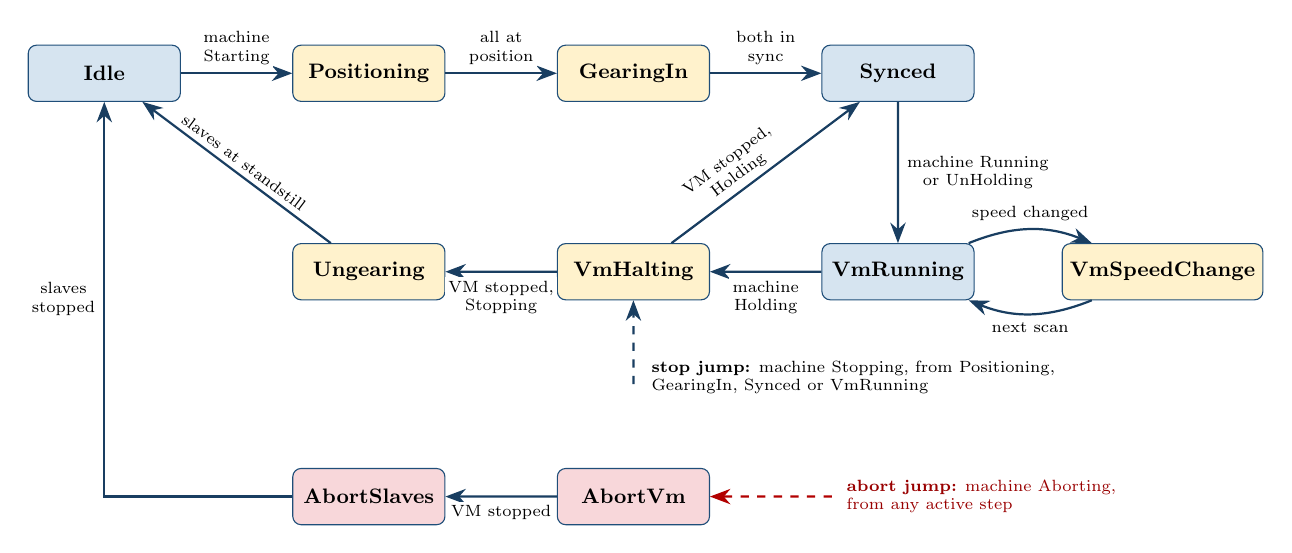
\begin{tikzpicture}[x=1cm,y=1cm,scale=0.84,transform shape]
  \node[sstate] (idle) at (0,0)       {Idle};
  \node[tstate] (pos)  at (4.0,0)     {Positioning};
  \node[tstate] (gin)  at (8.0,0)     {GearingIn};
  \node[sstate] (syn)  at (12.0,0)    {Synced};
  \node[tstate] (ung)  at (4.0,-3.0)  {Ungearing};
  \node[tstate] (halt) at (8.0,-3.0)  {VmHalting};
  \node[sstate] (run)  at (12.0,-3.0) {VmRunning};
  \node[tstate] (spd)  at (16.0,-3.0) {VmSpeedChange};
  \node[astate] (asl)  at (4.0,-6.4)  {AbortSlaves};
  \node[astate] (avm)  at (8.0,-6.4)  {AbortVm};

  \draw[tr] (idle) -- node[lbl,above=2pt]{machine\\Starting} (pos);
  \draw[tr] (pos) -- node[lbl,above=2pt]{all at\\position} (gin);
  \draw[tr] (gin) -- node[lbl,above=2pt]{both in\\sync} (syn);
  \draw[tr] (syn) -- node[lbl,right=2pt]{machine Running\\or UnHolding} (run);
  \draw[tr] (run) to[bend left=22] node[lbl,above=2pt]{speed changed} (spd);
  \draw[tr] (spd) to[bend left=22] node[lbl,below=2pt]{next scan} (run);
  \draw[tr] (run) -- node[lbl,below=2pt]{machine\\Holding} (halt);
  \draw[tr] (halt) -- node[lbl,sloped,above=1pt,pos=0.4]{VM stopped,\\Holding} (syn);
  \draw[tr] (halt) -- node[lbl,below=2pt]{VM stopped,\\Stopping} (ung);
  \draw[tr] (ung) -- node[lbl,sloped,above=1pt,pos=0.5]{slaves at standstill} (idle);
  \draw[tr] (avm) -- node[lbl,below=2pt]{VM stopped} (asl);
  \draw[tr] (asl.west) -| node[lbl,pos=0.75,left=2pt]{slaves\\stopped} (idle.south);

  % jumps
  \draw[tr,dashed] (8.0,-4.7) -- (halt.south);
  \node[font=\scriptsize,align=left,anchor=west] at (8.15,-4.6)
     {\textbf{stop jump:} machine Stopping, from Positioning,\\GearingIn, Synced or VmRunning};
  \draw[tr,dashed,draw=red!70!black] (11.0,-6.4) -- (avm);
  \node[font=\scriptsize,text=red!60!black,align=left,anchor=west] at (11.1,-6.4)
     {\textbf{abort jump:} machine Aborting,\\from any active step};
\end{tikzpicture}
\caption{Motion sequence. Dashed: jumps evaluated before the transitions.}
\end{figure}

\subsection{Behaviour notes}

\begin{itemize}
  \item \textbf{Gearing is absolute, to the VM's set point.} The slave's command is the VM's
        set point $\times\,1$ + the slave offset, so the gearing \emph{enforces} the phase.
        Positioning has already put the slaves at their offsets with the VM at 0, so gear-in
        needs no correction move. If a slave is ever out of phase, it's pulled back the shortest
        way.
  \item \textbf{Speed changes apply on the fly} in VmRunning, including during UnHolding,
        without stopping the VM. Where the library can't update a running velocity command, the
        one-scan \code{VmSpeedChange} state re-triggers it through the state machine. No edges are
        needed. The command must be one that keeps the VM moving while it's re-triggered.
  \item \textbf{Abort deceleration} (\code{ABORT_DEC}) is separate from the normal VM
        deceleration (\code{VM_DEC}). While geared, the slaves follow the VM down at whichever
        deceleration the VM is using.
  \item \textbf{A fault while running:} the drive's own error reaction stops the faulted axis.
        The machine aborts, AbortVm brings the VM down at \code{ABORT_DEC}, and the healthy slave
        follows it down while geared. AbortSlaves then ends the gearing. A faulted axis counts as
        stopped, so the abort can't hang on it.
\end{itemize}

\subsection{Echo and done per machine state}

\begin{center}
\begin{tabularx}{\linewidth}{P{4.4cm} L}
\toprule
\textbf{Machine state} & \textbf{Done when the sequence is in} \\
\midrule
\st{Starting} & \code{Synced} \\
\st{Holding} & \code{Synced} (VM stopped, still geared) \\
\st{UnHolding} & \code{VmRunning} and the VM at the commanded speed. If the speed changes mid-UnHolding, done drops until the new speed is reached. \\
\st{Stopping} & \code{Idle} (VM stopped, gearing ended, all at standstill) \\
\st{Aborting} & \code{Idle} (VM stopped, gearing aborted, all stopped) \\
Off, TurningOn, Idle, Running, Hold, Aborted, Resetting & Immediately: no motion work \\
\bottomrule
\end{tabularx}
\end{center}

The block echoes the machine state on the scan after its own transition logic has seen it. The
manager ignores done while the echo is still the old state (\S\ref{sec:clients}).

\section{Unit interface}\label{sec:servo-if}

\begin{xltabular}{\linewidth}{P{4cm} L}
\toprule
\textbf{Input} & \textbf{Meaning} \\
\midrule
\code{eMachineState} & The machine state to follow, wired by the calling program \\
\code{lrSpeedCmd} & VM velocity, in VM units/s. It can change at any time. \textbf{Limiting it is the caller's job}, so the unit doesn't clamp it. \\
\code{lrAx1Offset}, \code{lrAx2Offset} & Slave phase offsets from the VM, used both as the positioning targets and as the gear-in slave offsets. They're supplied by the caller. \\
Axis references & \code{Ax1}, \code{Ax2}, \code{VM}, of whatever axis reference type the chosen library uses \\
Axis cyclic status & Per axis (Ax1, Ax2, VM): ready for power, powered, standstill, error, in sync, data valid, from the motion system. The drive status words are \textbf{not} inputs; the drive hardware station owns them. \\
Client attachments & Two \code{I_StateClient}s, one per block, e.g.\ \code{GVL_State.aClients[CLIENT_SERVO_AXES]} and \code{[CLIENT_SERVO_MOTION]} \\
\bottomrule
\end{xltabular}

Outputs (diagnostics, copied from internal variables): \code{eSeqState}, the per-axis status
summary, and the abort code this unit raised.

\section{Constants}

\begin{center}
\begin{tabularx}{\linewidth}{P{6.4cm} L}
\toprule
\textbf{Constant} & \textbf{Meaning} \\
\midrule
\code{POS_VEL}, \code{POS_ACC}, \code{POS_DEC} & Dynamics for the start positioning moves \\
\code{VM_ACC}, \code{VM_DEC} & Normal VM ramp for run, hold and stop \\
\code{ABORT_DEC} & Abort deceleration for the VM and slaves. It's separate from \code{VM_DEC}. \\
\code{ABORT_AXIS_ERROR}, \code{ABORT_POWER_LOST}, \code{ABORT_MOTION_CMD} & Base abort codes. The axis or command index is added to them. \\
\bottomrule
\end{tabularx}
\end{center}

The machine-level timeouts for TurningOn, Starting, Stopping and the others live in the central
manager. They must allow for the longest positioning move.

\section{Decisions and assumptions}\label{sec:servo-decisions}

\textbf{\decided:}
\begin{enumerate}
  \item Positioning takes the \textbf{shortest way}.
  \item Gearing is \textbf{absolute, to the VM's set point}, with the slave offsets applied by the
        gearing itself.
  \item Abort uses its \textbf{own deceleration}, separate from the normal ramp.
  \item \textbf{Speed changes on the fly}, in Running and UnHolding.
  \item \textbf{Any fault aborts.} There are no partial or local stops.
  \item \textbf{The caller limits the speed command.} The unit doesn't clamp it.
  \item \textbf{The caller supplies the slave offsets.}
  \item \textbf{The design is library-agnostic.} The motion library is chosen at implementation
        time.
  \item \textbf{Torque-free at the end of Aborting.} Once all axes are at rest they're commanded
        torque-free while still in Aborting, so the drive supply can shut down before Aborted.
  \item \textbf{Power readiness comes from the axis's ready-for-power feedback}, not the drive
        status word, so any axis can be switched to a virtual axis for testing.
\end{enumerate}

\textbf{\assumed\ (please confirm):}
\begin{enumerate}
  \item The axes use absolute encoders, so no homing is needed before positioning in Starting.
  \item All three axes are modulo 360\textdegree.
  \item In Hold, the slaves stay geared, and only the VM stops.
  \item The offsets don't change while geared. If they can, the gear-in offset has to be one
        the library can update live.
\end{enumerate}

% =====================================================================
\chapter{Unit: Drive Hardware Station}\label{ch:drive}

\section{Purpose and scope}

The drive hardware station manages the \textbf{drive power supply}, the DC bus that feeds the
servo drives. It's one block, \code{FB_DriveSupplyMgr}, with one state client
(\code{FB_StateRequest}). It follows the machine state it's given as its \code{eMachineState}
input, wired by the calling program to the broadcast \code{GVL_State.eMachineState}.

\textbf{It owns:}
\begin{itemize}
  \item switching the supply on, but only once every drive reports it's ready for power;
  \item switching the supply off, but only once no axis is under torque;
  \item detecting a supply that doesn't come on, drops out or faults, and requesting an abort for
        it;
  \item waiting in Resetting for supply and drive faults to clear. The reset itself is the drive
        reset of drive 0, which hosts the supply, issued by the servo station.
\end{itemize}

\textbf{It does not own:} axis power or torque. That belongs to the servo station's axis
manager. The two units never talk to each other. This unit reads the drive status words, and the
servo station reads its axes' ready-for-power feedback from the motion system. That's enough to
order them correctly (\S\ref{sec:ordering}).

As with the other units, this design is library-agnostic. The supply command, supply feedback
and drive status words are plain signals, mapped from whatever I/O the hardware provides.

\section{Drive status word: bits 15/14 and bit 13}

Every axis drive reports its readiness in bits 15 and 14 of its status word:

\begin{center}
\begin{tabular}{c c l l}
\toprule
\textbf{Bit 15} & \textbf{Bit 14} & \textbf{Meaning} & \textbf{Used as} \\
\midrule
0 & 0 & Not ready for power & Blocks power-on \\
0 & 1 & Ready for power & \textbf{Ready for power} (bit 14 or bit 15 set) \\
1 & 0 & Power section ready, torque-free & Ready for power, not under torque \\
1 & 1 & Under torque & \textbf{Under torque} (bit 14 and bit 15 set) \\
\bottomrule
\end{tabular}
\end{center}

Two derived levels, taken across all axis drives:
\begin{itemize}
  \item \code{bAllReadyForPower := every drive has (bit 14 OR bit 15)}
  \item \code{bAnyUnderTorque := any drive has (bit 14 AND bit 15)}
\end{itemize}

\textbf{Bit 13 is the fault bit.} It's checked on every axis drive's status word and on the
\textbf{supply's own status word}:
\begin{itemize}
  \item \code{bAnyDriveFault := any drive has bit 13}
  \item \code{bSupplyFault := supply status word bit 13}
\end{itemize}

\section{Behaviour per machine state}

\begin{xltabular}{\linewidth}{P{3.6cm} L P{3.8cm}}
\toprule
\textbf{Machine state} & \textbf{Supply} & \textbf{Done when} \\
\midrule
\st{Off} & Off, once no axis is under torque & Supply off \\
\st{TurningOn} & On, once all drives are ready for power & Supply on \\
Idle, Starting, Running, Stopping, Holding, Hold, UnHolding & On & Immediately: nothing to do beyond staying on \\
\st{Aborting} & Stays on until \textbf{no axis is under torque}, then off & No axis under torque \textbf{and} supply off \\
\st{Aborted} & Off & Immediately \\
\st{Resetting} & Reset supply and drive faults, then on once all drives are ready for power & No faults \textbf{and} supply on \\
\bottomrule
\end{xltabular}

\subsection*{The supply command as one level rule}

\begin{lstlisting}
bWantOn     := eMachineState <> Off AND eMachineState <> Aborted
               AND eMachineState <> Aborting;
// switch on only when all drives are ready, then stay on ...
_bSupplyCmd := (bWantOn AND (_bSupplyCmd OR bAllReadyForPower))
// ... and never switch off while any axis is under torque
               OR (_bSupplyCmd AND bAnyUnderTorque);
\end{lstlisting}

\begin{itemize}
  \item \textbf{Ready check, at switch-on only.} Once the supply is on, the drives move to
        ``power section ready'' or ``under torque''. Both still count as ready, and the supply
        holds itself on.
  \item \textbf{Torque check, at switch-off.} This applies to any switch-off, whether to Off or
        in Aborting. The supply goes off only after every axis is torque-free.
  \item \code{_bSupplyCmd} is internal. Reading its value from the previous scan is a self-hold,
        not a read of an output.
\end{itemize}

\section{Ordering with the servo station, via hardware status only}\label{sec:ordering}

\begin{xltabular}{\linewidth}{P{2.6cm} L L}
\toprule
\textbf{Phase} & \textbf{Drive hardware station} & \textbf{Servo axis manager} \\
\midrule
TurningOn / Resetting & Waits until all drives are \emph{ready for power}, then switches the supply on & Waits until each axis reports \emph{ready for power} (motion feedback, which follows the DC bus for a real axis), then enables the axes \\
Aborting & Holds the supply on while any axis is \emph{under torque}, then switches off & Stops the axes, then commands them \textbf{torque-free} once at rest, still in Aborting \\
Off & Switches off once no axis is under torque & Disables the axes \\
\bottomrule
\end{xltabular}

\begin{figure}[h]
\centering
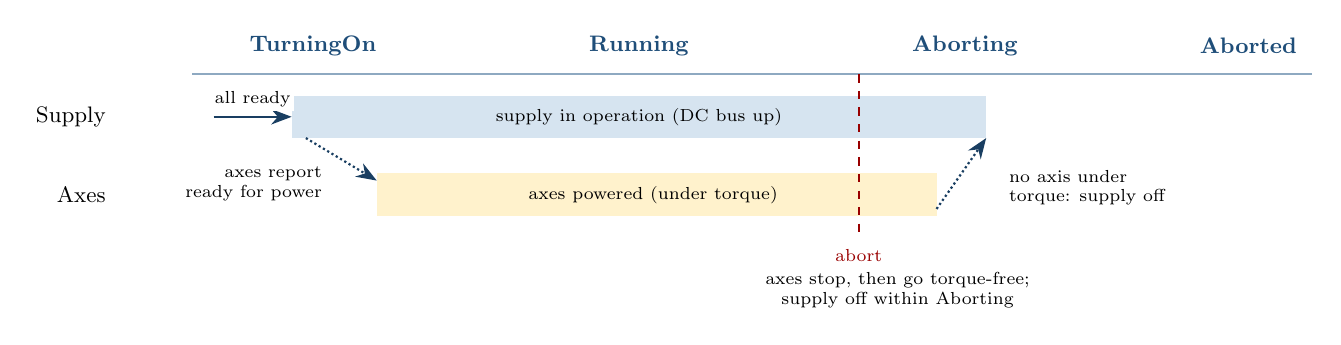
\begin{tikzpicture}[x=1cm,y=1cm,scale=0.9,transform shape]
  \foreach \x/\t in {0/TurningOn, 4.6/Running, 9.2/Aborting, 13.2/Aborted} {
    \node[font=\small\bfseries,text=accent] at (\x+1.5,1.0) {\t};
  }
  \draw[thick,draw=rule] (-0.2,0.6) -- (15.6,0.6);
  \node[anchor=east,font=\small] at (-1.3,0) {Supply};
  \node[anchor=east,font=\small] at (-1.3,-1.1) {Axes};
  % supply
  \fill[stable] (1.2,-0.3) rectangle (11.0,0.3);
  \node[font=\scriptsize] at (6.1,0) {supply in operation (DC bus up)};
  \draw[tr] (0.1,0) -- node[lbl,above=2pt]{all ready} (1.2,0);
  % axes
  \fill[transitional] (2.4,-1.4) rectangle (10.3,-0.8);
  \node[font=\scriptsize] at (6.3,-1.1) {axes powered (under torque)};
  \draw[tr,densely dotted] (1.4,-0.3) -- (2.4,-0.9);
  \node[font=\scriptsize,align=right,anchor=east] at (1.75,-0.95) {axes report\\ready for power};
  \draw[tr,densely dotted] (10.3,-1.3) -- (11.0,-0.3);
  \node[font=\scriptsize,align=left,anchor=west] at (11.2,-1.0) {no axis under\\torque: supply off};
  \draw[thick,dashed,draw=red!60!black] (9.2,0.6) -- (9.2,-1.7);
  \node[font=\scriptsize,text=red!60!black] at (9.2,-1.95) {abort};
  \node[font=\scriptsize,align=center] at (9.75,-2.45) {axes stop, then go torque-free;\\supply off within Aborting};
\end{tikzpicture}
\caption{The units order themselves by hardware status alone. The supply comes up before the
axes power on, and goes down only after every axis is torque-free.}
\end{figure}

The machine can only leave \textbf{Aborting} when both units are done: the axes are torque-free
and the supply is off. \textbf{Aborted} is therefore reached with the bus already down.

\section{Fault detection: abort requests}

\textbf{Any fault aborts.} Outside Aborting, Aborted and Resetting (\S\ref{sec:jumps}), the
block requests an abort (through its client) while any of these is TRUE:

\begin{center}
\begin{tabularx}{\linewidth}{P{4.4cm} L}
\toprule
\textbf{Abort code} & \textbf{Condition} \\
\midrule
\code{ABORT_SUPPLY_CTRL} & The supply didn't reach the commanded mode in time (or its controller rejected the command) \\
\code{ABORT_SUPPLY_FAULT} & The supply reports an internal error, read from its status word. \textbf{This also covers a supply that drops out after it was on.} \\
\code{ABORT_DRIVE_FAULT + i} & Drive $i$ fault: drive $i$ status word bit 13 \\
\bottomrule
\end{tabularx}
\end{center}

\textbf{Only power-on aborts on time.} The supply controller supervises every mode change, on
and off. An off change only happens in Off, where the manager ignores aborts, or in Aborting,
where fault aborts aren't raised. So in practice only a supply that fails to come on causes an
abort. Once the supply is up, a drop-out shows as a supply fault.

There's no local timeout for drives that never become ready for power. The supply simply isn't
commanded, this client never reports done, and the manager's TurningOn or Resetting timeout
aborts with this client recorded as not done.

\section{Reset}

\textbf{This block doesn't reset anything itself.} The supply is built into drive 0, which is
Ax1's drive, so the \textbf{drive reset of drive 0} clears supply errors as well as drive
errors. The servo station's axis manager resets both axes on entry to Resetting, whatever the
fault was. Any fault aborts, so Resetting always follows a fault, and the reset doesn't need to
know which one.
\begin{itemize}
  \item This block waits in Resetting. When the faults clear, the drives report ready for power
        and the supply rule brings the supply back to operation.
  \item If the supply controller itself is in error, its enable is held off while Resetting,
        which clears it.
  \item The block is done when there are no faults and the supply is in operation.
  \item If the reset doesn't clear things, the manager's Resetting timeout aborts again.
\end{itemize}

\section{Interface}

\begin{xltabular}{\linewidth}{P{4cm} L}
\toprule
\textbf{Input} & \textbf{Meaning} \\
\midrule
\code{eMachineState} & The machine state to follow, wired by the calling program \\
\code{awDriveStatus} & Status words of the \textbf{drives in use} on this supply (array: drive 0 = Ax1, drive 1 = Ax2): bits 15/14 readiness, bit 13 fault. The spare drive 2 isn't included. \\
\code{wSupplyStatus} & Supply unit status word: operating mode and internal error \\
Client attachment & One \code{I_StateClient}, e.g.\ \code{GVL_State.aClients[CLIENT_DRIVE_HW]} \\
\midrule
\textbf{Output} & \textbf{Meaning} \\
\midrule
\code{wSupplyCtrl} & Supply unit control word (in/out): drives the supply to operation or mains off \\
\code{awDriveDcBusCtrl} & DC bus power control of each drive (in/out): ``DC bus power'' is set while the supply is in operation \\
Diagnostics & \code{bSupplyInOperation}, \code{bSupplyOff}, \code{bAllReadyForPower}, \code{bAnyUnderTorque}, \code{bAnyDriveFault}, \code{bSupplyFault}, the abort code raised \\
\bottomrule
\end{xltabular}

\textbf{Constants:}
\begin{itemize}
  \item \code{SUPPLY_MODE_TIMEOUT}: the longest a supply mode change may take
  \item \code{ABORT_SUPPLY_CTRL}, \code{ABORT_SUPPLY_FAULT}, \code{ABORT_DRIVE_FAULT}: abort codes
\end{itemize}

\section{Internal structure}

As with the servo axis manager, there's no internal state machine. Everything is a level
function of the machine state and the hardware status:
\begin{enumerate}
  \item read the status: decode each drive's status word with a sub-function (ready for power,
        under torque, fault), and read the supply's mode and error from its controller;
  \item fault conditions $\rightarrow$ abort request and code;
  \item echo and done from the machine state;
  \item command levels: \code{_bSupplyCmd} $\rightarrow$ supply target mode (operation / mains
        off), the supply controller's enable, and DC bus power to each drive;
  \item call the sub-FBs (supply controller, client wrapper), then copy the outputs last.
\end{enumerate}

\section{Decisions and assumptions}

\textbf{\decided:}
\begin{enumerate}
  \item Power-on is allowed only when every drive is \textbf{ready for power} (status bit 14 or
        15).
  \item A supply that doesn't power on means \textbf{abort}. \textbf{Only power-on aborts on
        time}. A drop-out after power-on is caught as a supply fault.
  \item In Aborting, the supply goes off only after \textbf{no axis is under torque} (bits 14 and
        15 not both set), and that happens \textbf{within Aborting}. The servo station makes its
        axes torque-free at the end of Aborting.
  \item Resetting \textbf{brings the supply back on} once the faults are cleared. \textbf{The
        reset is the drive reset of drive 0} (the supply is built into it), issued by the servo
        axis manager. This block has no reset output.
  \item \textbf{A supply or drive fault means abort}: a supply internal error, or bit 13 of any
        drive status word.
  \item \textbf{The supply is off in Off and Aborted, and on in every other state}, including
        Idle.
  \item \textbf{There are 3 drives and 1 supply.} Drive 0 is Ax1 and hosts the supply, and
        drive 1 is Ax2. These two get DC bus power while the supply is in operation.
        \textbf{Drive 2 is a spare and doesn't count}: it isn't part of readiness, torque or
        fault checks.
  \item \textbf{One supply feeds all 3 drives} (confirmed). The VM has no drive.
  \item \textbf{A drop-out is caught by the supply fault} (bit 13). Only power-on is timed.
\end{enumerate}

\end{document}
